\documentclass[11pt,border=4pt]{standalone}
\usepackage{amsmath,amssymb,bm,mathtools}
\usepackage[fontset=fandol]{ctex}
\usepackage{tikz}
\usetikzlibrary{arrows.meta,calc,patterns,angles,quotes,decorations.markings,decorations.pathmorphing}
\newcommand{\dd}{\mathop{}\!\mathrm d}
\newcommand{\e}{\mathrm e}
\tikzset{axis/.style={->,>=Stealth,line width=.45pt},world/.style={line width=.8pt},flow/.style={->,>=Stealth,line width=.7pt},ray/.style={->,>=Stealth,line width=.7pt},guide/.style={dashed,line width=.35pt},aux/.style={dashed,line width=.35pt},dim/.style={<->,>=Stealth,line width=.35pt},every node/.style={font=\small},force/.style={->,>=Stealth,very thick},gas/.style={fill=blue!7}}
\begin{document}
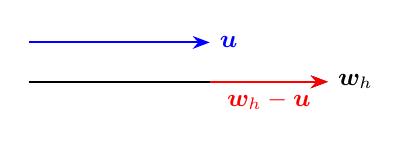
\begin{tikzpicture}\draw[flow](0,0)--(3.8,0)node[right]{$\bm w_h$};\draw[flow,blue](0,.5)--(2.3,.5)node[right]{$\bm u$};\draw[flow,red](2.3,0)--(3.8,0)node[midway,below]{$\bm w_h-\bm u$};\end{tikzpicture}
\end{document}
